\section{Атака на алгоритм шифрования RSA посредством метода Ферма}

\textbf{Цель работы}: изучить атаку на алгоритм шифрования RSA посредством метода Ферма.

Дано: $N=84032429242009$, $e=2581907$, $c=\seqsplit{%
	54879925681459
	72167008182929
	17828219756166
	17814399744948
	37136636080011
	77223434260215
	4272415279426
	73759271926435
	74021335775875
	16903113250201
	77520052156956
	41247980943013}$.

\begin{enumerate}
	\item Вычисляем $n = \sqrt{N} + 1$. В поле A помещаем $N$, в поле B $–2$; нажимаем кнопку <<D = A\^(1/B)>>. В поле D заносится число 9166921. В первой строке таблицы появляется сообщение <<[error]>>. Это свидетельствует о том, что $N$ не является квадратом целого числа.
	
	
	\item $t_1 = n + 1$. Возводим число $t_1$ в квадрат: A: = 9166922, B: = 2, C: = 0 (возведение в квадрат будет производиться не по правилам модульной арифметики), нажимаем <<D = A$\^$B mod C>> => D = t1$\^$2 = 84032458954084. Вычисляем w1 = t1$\^$2 – N. Для этого A:= t1$\^$2, B:= –N, затем нажимаем <<D = A + B>> => D = w1 = 29712075. Проверяем, является ли w1 квадратом целого числа: A:= w1, B:= 2, нажимаем <<D = A$\^$(1/B)>> => в первой строке таблицы появляется сообщение <<[error]>>.
	
	
	\item При вычислении квадратного корня w4 первая строка таблицы остается пустой, а D = sqrt(w4) = r, что свидетельствует об успехе факторизации. t4 = 9166925.
	
	
	\item Вычисляем p = t4 + sqrt(w4); A:= t4, B:= sqrt(w4), нажимаем <<D = A + B>>  => D = p = 9176129; q = t4 – sqrt(w4) = 9157721. Вычисляем Phi(N) = (p – 1)(q – 1), A:= 9176128, B:= 9157720, нажимаем <<D = A $\cdot$ B>> => D = Phi(N) = 84032410908160. Вычисляем d, как обратный к e: A:= e, B:= –1, C:= Phi(N), нажимаем <<D = A $\^$ B mod C>> => D = d = 2475823295643.
	
	
	\item Производим дешифрацию шифрблока С: A:= C; B:= d; C:= N. Нажимаем <<D = A $\^$ B mod C>>. В поле D находится исходное сообщение M. Переводим M в текстовый вид. Для этого A:= M, нажимаем <<D = text(A)>>. Повторяем с каждым шифроблоком.

\end{enumerate}



\begin{figure}[H]
	\centering
	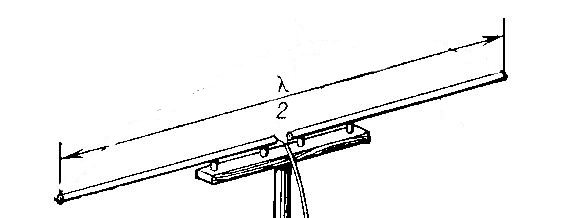
\includegraphics[width=0.7\linewidth]{img/1}
	\caption{Результат работы программы BCalc}
\end{figure}


